\documentclass{article}
\usepackage[T1]{fontenc}
\usepackage[utf8]{inputenc}
\usepackage[a4paper, total={6in, 11in}]{geometry}
\usepackage{algorithm}
\usepackage{amsfonts}
\usepackage{algpseudocode}
\usepackage{float}
\usepackage{graphicx}
\usepackage{subcaption}

\def\v{0.47}

\title{%
	Obliczenia naukowe \\
	\large Lista 2}
\author{Szymon Janiak}
\begin{document}
\maketitle

\section*{Zadanie 1}
\subsection*{Opis problemu}
    Obliczenie iloczynu skalarnego róznymi funkcjami dwóch wektorów i porównanie wyników przy lekkiej zmianie danych wejściowych
\subsection*{Rozwiązanie}
    \begin{enumerate}
        \item "w przód" t.j. $\sum^n_{i=1} x_i y_i$
        \item "w tył" t.j. $\sum^1_{i=n} x_i y_i$
        \item "liczby dodatnie od najwiekszego do najmniejszego a ujemne na odwrót"
        \item "liczby ujemne od najwiekszego do najmniejszego a dodatnie na odwrót"
    \end{enumerate}
\subsection*{Wyniki}
    \begin{center}
        \begin{tabular}{|c|c|c|c|}
        \hline
            & Float64 stare dane & Float64 nowe dane & Prawidłowy wynik \\
            \hline\hline
            "1" & 1.0251881368296672e-10 & -0.004296342739891585 & -1.00657107000000e-11 \\
             \hline
             "2" & -1.5643308870494366e-10 & -0.004296342998713953 & -1.00657107000000e-11 \\
             \hline
             "3" & 0.0 & -0.004296342842280865 & -0.004296342842280865 \\
             \hline
             "4" & 0.0 & -0.004296342842280865 & -0.004296342842280865 \\
        \hline
        \end{tabular}
    \end{center}
\subsection*{Wnioski}
	Przy usunięciu ostatniej 9 z $x_4$ oraz ostatniej 7 z $x_5$ dostajemy różne wyniki dla podwójnej precyzji.
	Po tak lekkiej zmianie danych możemy zauważyć, że wyniki dla wszystkich funkcji są znacznie bardziej przybliżone, prawie identyczne.
	Dla Float32 nie ma żadnej różnicy, gdyż jest to za mała precyzja. Według definicji jest to źle uwarunkowane zadanie.

\section*{Zadanie 2}
\subsection*{Opis problemu}
	Narysować wykres funkcji $f(x) = e^xln(1 + e^{-x})$ w co najmniej dwóch dowolnych programach do wizualizacji. \\
	Porównać wykres funkcji z policzoną granicą dla funkcji $\lim_{x\to\infty}f(x)$.
\subsection*{Wyniki}
	\begin{figure}[H]
		\centering
		\begin{subfigure}[b]{\v\linewidth}
			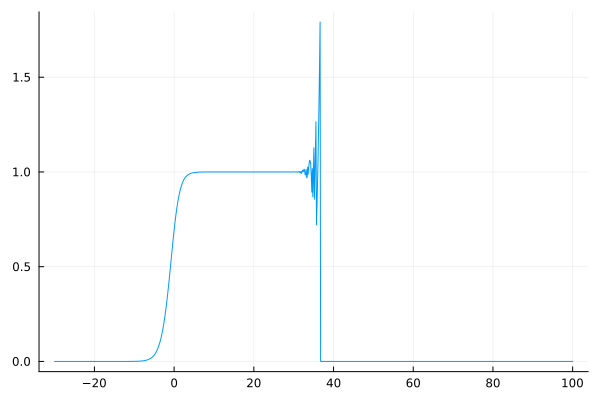
\includegraphics[width=\linewidth]{graphs/2.1.png}
			\caption{Biblioteka Plots w języku Julia}
			\label{fig:enter-label}
		\end{subfigure}
		\begin{subfigure}[b]{\v\linewidth}
			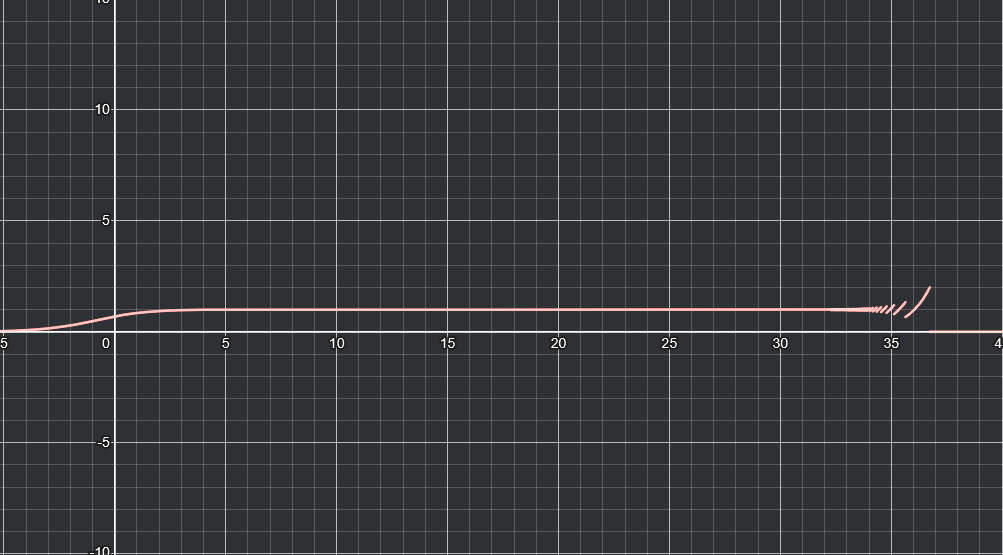
\includegraphics[width=\linewidth]{graphs/2.2.png}
			\caption{Desmos}
			\label{fig:enter-label}
		\end{subfigure}
	\end{figure}
	Poniżej policzona granica: \\
	\[\lim_{x\to\infty}e^xln(1+e^{-x})=\lim_{x\to\infty}\frac{ln(1+e^{-x})}{e^{-x}}=\lim_{x\to\infty}\frac{-e^{-x}}{(1+e^{-x})*(-e^{-e})}=\lim_{x\to\infty}\frac{1}{1+e^{-x}}=1\]

\subsection*{Wnioski}
	Widzimy na wykresach, że w okolicach $x = 30$ pojawiają się problemy z obliczaniem wartości naszej funkcji. \\
	Mimo, że funkcja dąży do 1 nasze programy mają wyraźny problem z obliczaniem wartości składających się na wynik naszej funkcji.
	Jest to prawdopodobnie spowodowane brakiem wystarczającej precyzji kiedy wartości $e^{-x}$ robią się coraz mniejsze.

\section*{Zadanie 3}
\subsection*{Opis problemu}
	Rozważmy zadanie rozwiązywania układu równań liniowych \\
	\centerline{$Ax = b$}
	dla danej macierzy współczynników $A \in \mathbb{R}^{n\times n}$ i wektora prawych stron $b \in \mathbb{R}^{n}$
\subsection*{Wyniki}
	\begin{center}
        \begin{tabular}{|c|c|c|c|c|}
        \hline
        n & rank & cond & odwrotna & gauss \\
        \hline
		1 & 1 & 1.0 & 0.0 & 0.0\\
		\hline
		3 & 3 & 524.0567775860627 & 9.825526038180824e-15 & 8.351061872731819e-15\\
		\hline
		5 & 5 & 476607.2502419338 & 8.128168770215688e-12 & 1.256825919192874e-12\\
		\hline
		7 & 7 & 4.753673568766496e8 & 4.3299229851434615e-9 & 6.520804933066021e-9\\
		\hline
		9 & 9 & 4.9315332284138226e11 & 1.4626798972086921e-5 & 1.3216991540025553e-5\\
		\hline
		11 & 10 & 5.224780779168285e14 & 0.010645959401385671 & 0.01004906783345069\\
		\hline
		13 & 11 & 4.4936679531246986e18 & 82.66675811171989 & 70.1556197115221\\
		\hline
		15 & 12 & 3.3660126672602944e17 & 715.740988667373 & 692.4295360390742\\
		\hline
		17 & 12 & 6.26204622473199e17 & 17.157982115668773 & 18.67581817300634\\
		\hline
		19 & 13 & 3.462302955915255e18 & 16.84769281513296 & 15.073941146224387\\
		\hline
		21 & 13 & 1.1932537352623989e19 & 2333.664337044678 & 1824.2629581352649\\
		\hline
		23 & 13 & 1.2225550561673262e18 & 47.65132347528787 & 48.016565072622186\\
		\hline
		25 & 13 & 3.831285828118405e20 & 52.47720466798266 & 24.17187724650818\\
		\hline
		27 & 14 & 8.174081570715539e18 & 132.55118714543525 & 55.63396491601018\\
		\hline
		29 & 14 & 3.802856907227447e20 & 18.082557101050654 & 25.888760818983354\\
		\hline
		\end{tabular}
	\end{center}
	Wyniki dla macierzy Hilberta

	\begin{center}
        \begin{tabular}{|c|c|c|c|c|}
        \hline
        n & rank & cond & odwrotna & gauss \\
		\hline
		5 & 5 & 1.0000000000000007 & 1.4043333874306804e-16 & 1.85775845048325e-16\\
		\hline
		5 & 5 & 10.000000000000002 & 2.0471501066083611e-16 & 1.719950113979703e-16\\
		\hline
		5 & 5 & 999.9999999999818 & 3.727189175310957e-14 & 3.770981636172923e-14\\
		\hline
		5 & 5 & 1.0000000004525637e7 & 9.850842115240043e-11 & 1.2882333343613825e-10\\
		\hline
		5 & 5 & 1.0000800330968911e12 & 1.9973430651815224e-5 & 1.7562984167111192e-5\\
		\hline
		5 & 4 & 8.826715821066153e15 & 0.026083060333373865 & 0.04168369996461502\\
		\hline
		10 & 10 & 1.0000000000000016 & 2.1355566272775288e-16 & 2.6506211417561425e-16\\
		\hline
		10 & 10 & 10.0 & 2.9996574304705467e-16 & 2.1925147983971603e-16\\
		\hline
		10 & 10 & 999.9999999999974 & 2.54306514045846e-14 & 2.3210725195019588e-14\\
		\hline
		10 & 10 & 9.999999993688306e6 & 2.0614295394758574e-10 & 2.6921505988726474e-10\\
		\hline
		10 & 10 & 1.0000779893498125e12 & 2.1604172649799173e-5 & 2.3309127440445607e-5\\
		\hline
		10 & 9 & 8.26371308188777e15 & 0.05207598489435024 & 0.04340810877472368\\
		\hline
		20 & 20 & 1.0000000000000009 & 4.1836409184574146e-16 & 5.85372920201624e-16\\
		\hline
		20 & 20 & 10.000000000000009 & 5.336004900468223e-16 & 5.153874832879506e-16\\
		\hline
		20 & 20 & 999.9999999999743 & 5.444577179721357e-14 & 5.3415984214944754e-14\\
		\hline
		20 & 20 & 1.0000000003501127e7 & 3.3063603819760504e-11 & 1.2531568083980406e-11\\
		\hline
		20 & 20 & 9.999177938109891e11 & 4.710803617564571e-6 & 3.5356514545986903e-6\\
		\hline
		20 & 19 & 1.0095702285935152e16 & 0.21424321252672052 & 0.2140080771811224\\
		\hline
		\end{tabular}
	\end{center}
	Wyniki dla macierzy losowej
\subsection*{Wnioski}
	Uwarunkowanie macierzy $cond$ ma spory wpływ na skale otrzymywanych pomyłek.\\
\section*{Zadanie 4}
\subsection*{Opis problemu}
	Użyć funkcji $roots$ (z pakietu Polynomials) do obliczenia 20 zer wielominau $P$ w postaci naturalnej. \\
	$P$ jest postacią naturalną wielomianu Wilkinsona $p$ \\
	$p(x) = (x - 20)(x - 19)(x - 18)(x - 17)(x - 16)(x - 15) \\
			(x - 14)(x - 13)(x - 12)(x - 11)(x - 10)(x - 9) \\
			(x - 8)(x - 7)(x - 6)(x - 5)(x - 4)(x - 3)(x - 2)(x - 1)$
\subsection*{Wyniki}
	\begin{figure}[H]
		\centering
		\begin{subfigure}[b]{\v\linewidth}
			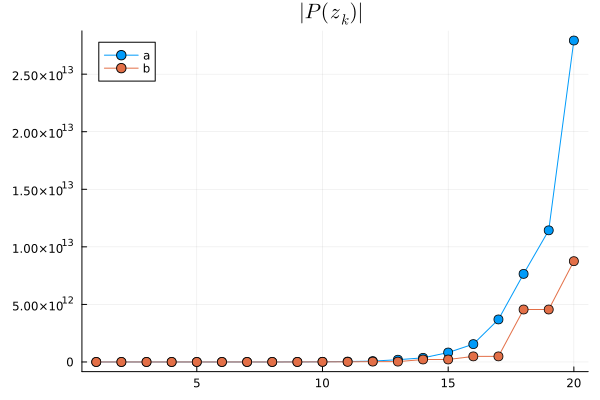
\includegraphics[width=\linewidth]{graphs/4.1.png}
		\end{subfigure}
		\begin{subfigure}[b]{\v\linewidth}
			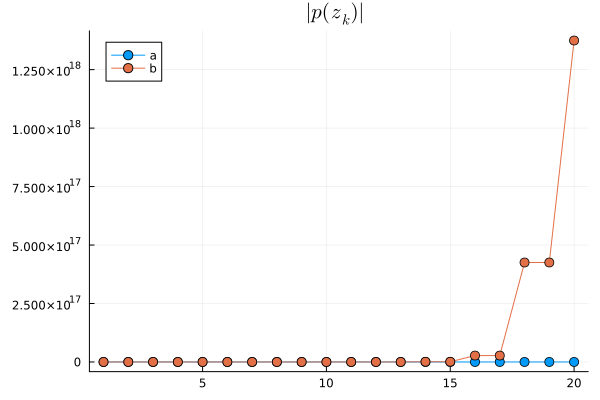
\includegraphics[width=\linewidth]{graphs/4.2.png}
		\end{subfigure}
		\begin{subfigure}[b]{\v\linewidth}
			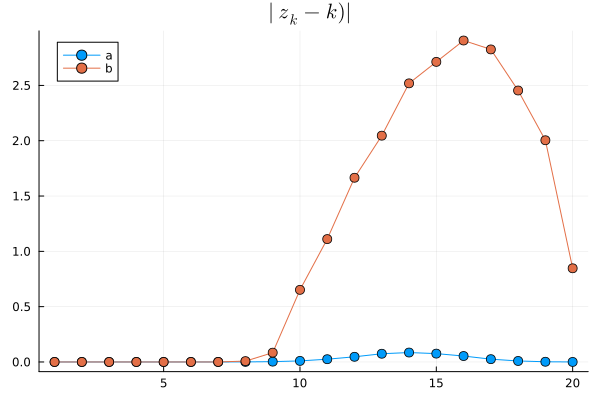
\includegraphics[width=\linewidth]{graphs/4.3.png}
		\end{subfigure}
	\end{figure}
\subsection*{Wnioski}
	Po wykresach widać, że obliczone przez nas miejsca zerowe nie pokrywają się z rzeczywistością. \\
	Wynika to z ograniczeń arytmetyki w Float64, która ma od 15 do 17 cyfr znaczących w systemie dziesiętnym. \\
	Po modyfikacji jednego współczynnika rozbieżności mogą być jeszcze większe.

\section*{Zadanie 5}
\subsection*{Opis problemu}
	Rozważmy równanie rekurencyjne \\
	\centerline{$p_{n+1} := p_n^2 + rp_n(1 - p_n)$ dla $n = 0, 1...,$ \\}
	gdzie $r$ jest pewną daną stałą, $r(1 - p_n)$ jest czynnikiem wzrostu populacji, a $p_0$ jest wielkością populacji stanowiącą procent maksymalnej wielkości populacji dla danego stanu środowiska. \\
	Przeprowadzić następujące eksperymenty:
	\begin{enumerate}
        \item Dla danych $p_0 = 0.01$ i $r = 3$ wykonać 40 iteracji wyrażenia (1), a następnie wykonać ponownie 40 iteracji wyrażenia (1) z niewielką modyfikacją tj. wykonać 10 iteracji, zatrzymać, zastosować obcięcie wyniku odrzucając cyfry po trzecim miejscu po przecinku (daje to liczbę 0.722) i kontynuować dalej obliczenia (do 40-stej iteracji) tak, jak gdyby był to ostatni wynik na wyjściu. Porównać otrzymane wyniki.
        \item Dla danych $p_0 = 0.01$ i $r = 3$ wykonać 40 iteracji wyrażenia (1) w arytmetyce Float32 i Float64. Porównać otrzymane wyniki.
    \end{enumerate}
\subsection*{Wyniki}
	\begin{figure}[H]
		\centering
		\begin{subfigure}[b]{\v\linewidth}
			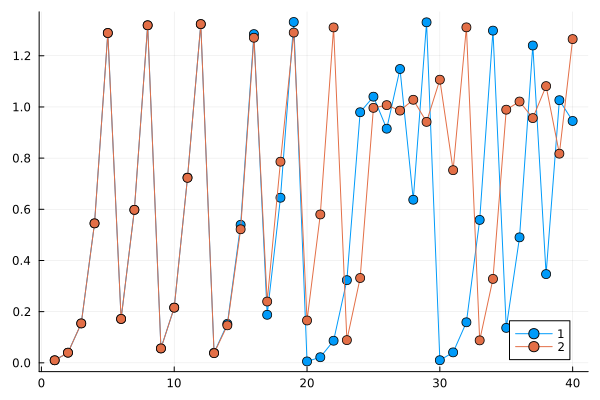
\includegraphics[width=\linewidth]{graphs/5.1.png}
		\end{subfigure}
		\begin{subfigure}[b]{\v\linewidth}
			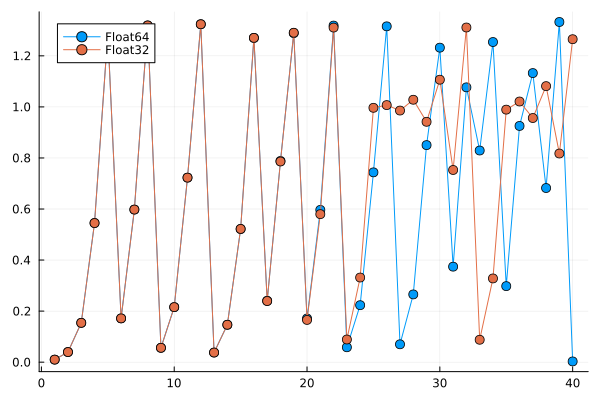
\includegraphics[width=\linewidth]{graphs/5.2.png}
		\end{subfigure}
	\end{figure}
\subsection*{Wnioski}
	W pierwszym eksperymencie możemy zauważyć, że obcięcie wyniku do 3 miejsc po przecinku powoduje po chwili znaczne rozjechanie się wyników. \\
	W drugim eksperymencie zjawisko jest podobne, większa precyzja pozwala na dokładniejsze wyniki, co również powoduje znaczne rozjechanie się wyników. \\
	Pokazuje to jak bardzo wyniki naszych obliczeń mogą się różnić w zależności od odpowiednio dobranej precyzji.

\section*{Zadanie 6}
\subsection*{Opis problemu}
	Dla równania rekurencyjnego \\
	\centerline{$x_{n+1} := x_n^2 + c$ dla $n = 0, 1...,$ \\}
	Przeprowadzić następujące eksperymenty. Dla danych:
	\begin{enumerate}
        \item $c = -2$ i $x_0 = 1$
        \item $c = -2$ i $x_0 = 2$
        \item $c = -2$ i $x_0 = 1.99999999999999$
        \item $c = -1$ i $x_0 = 1$
        \item $c = -1$ i $x_0 = -1$
        \item $c = -1$ i $x_0 = 0.75$
        \item $c = -1$ i $x_0 = 0.25$
    \end{enumerate}
    wykonać w arytmetyce Float64, 40 iteracji podanego wyrażenia i przeprowadzić iteracje graficzną.
\subsection*{Wyniki}
	\begin{figure}[H]
		\centering
		\begin{subfigure}[b]{\v\linewidth}
			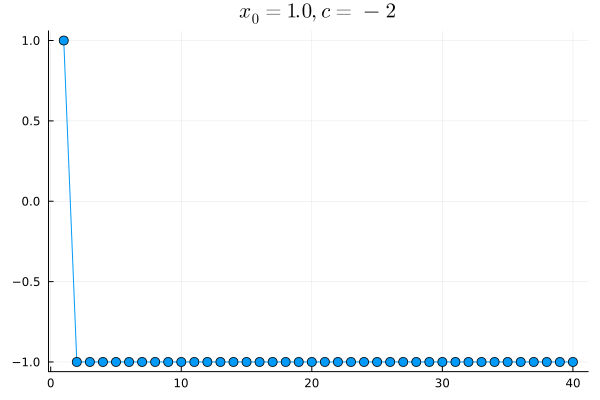
\includegraphics[width=\linewidth]{graphs/1.png}
		\end{subfigure}
		\begin{subfigure}[b]{\v\linewidth}
			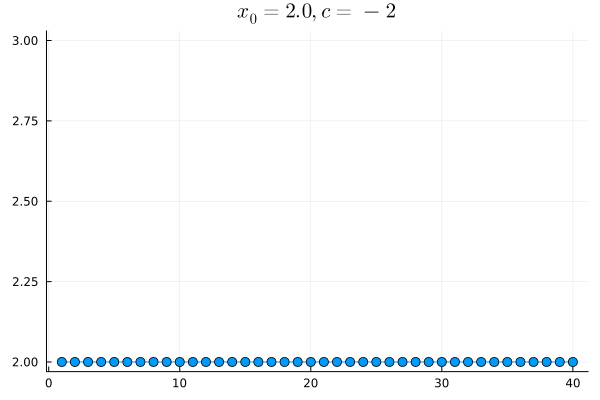
\includegraphics[width=\linewidth]{graphs/2.png}
		\end{subfigure}
		\begin{subfigure}[b]{\v\linewidth}
			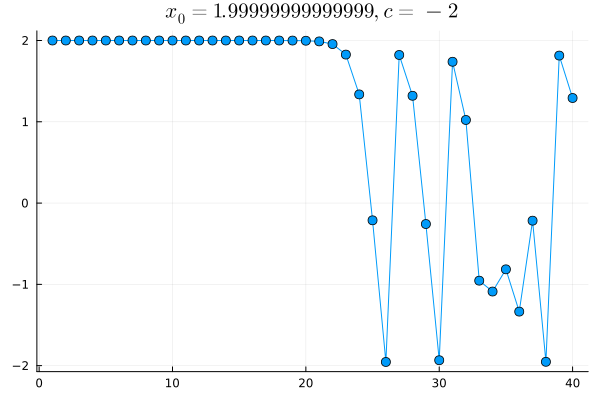
\includegraphics[width=\linewidth]{graphs/3.png}
		\end{subfigure}
		\begin{subfigure}[b]{\v\linewidth}
			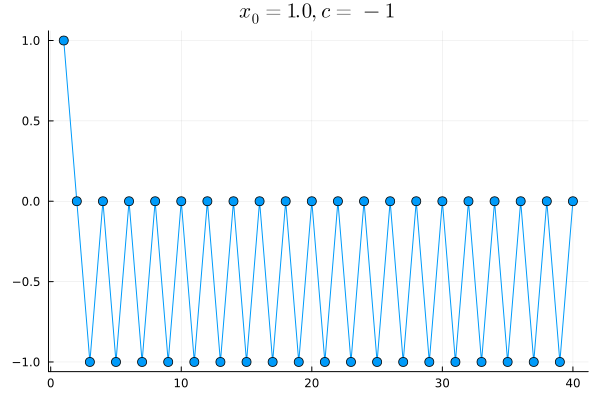
\includegraphics[width=\linewidth]{graphs/4.png}
		\end{subfigure}
		\begin{subfigure}[b]{\v\linewidth}
			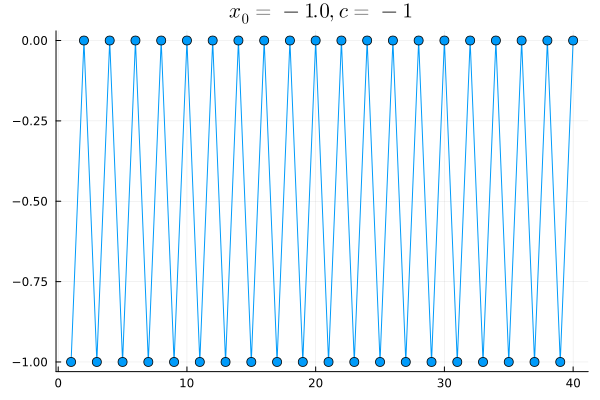
\includegraphics[width=\linewidth]{graphs/5.png}
		\end{subfigure}
		\begin{subfigure}[b]{\v\linewidth}
			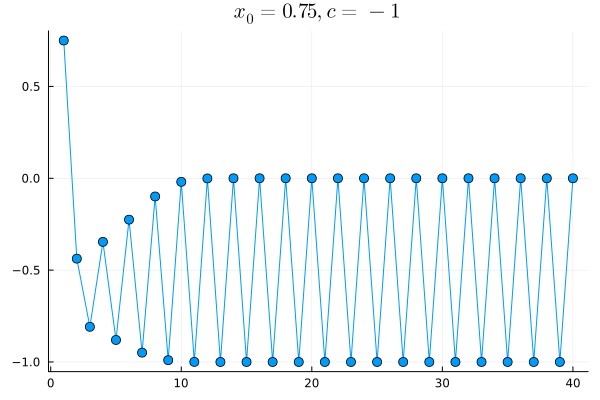
\includegraphics[width=\linewidth]{graphs/6.png}
		\end{subfigure}
		\begin{subfigure}[b]{\v\linewidth}
			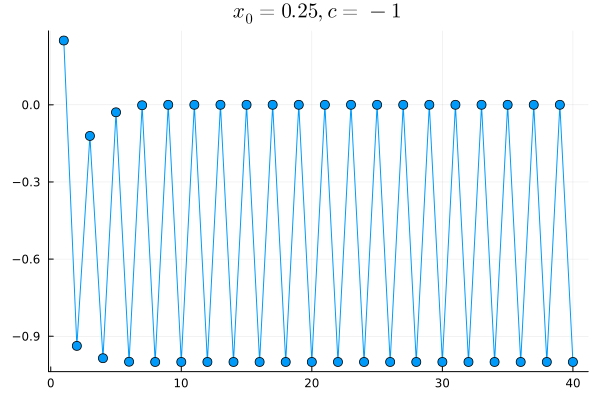
\includegraphics[width=\linewidth]{graphs/7.png}
		\end{subfigure}
	\end{figure}
\subsection*{Wnioski}
	Możemy zauważyć, że najciekawszym wykresem jest ten dla $x_0 = 1.999...$, wynika to z kumulujących się błędów obliczania precyzji.

\end{document}